\documentclass[a4paper]{article}

\usepackage[utf8]{inputenc}
\usepackage[T1]{fontenc}
\usepackage[norsk]{babel}
\usepackage{amsmath}
\usepackage{amssymb}
\usepackage{algorithmic}
\usepackage{authblk}
\usepackage{enumitem}
\usepackage{float}
\usepackage{graphicx}
\usepackage{libertine}
\usepackage[libertine]{newtxmath}

\title{Oversikt over algoritmer og metoder i TDT4120}
\author{Morten Fyhn Amundsen}
\affil{NTNU}

%Skriv i imperativ.
%Bruk seksjoner for kategorier av algoritmer.
%Skriv høynivå, tydelig, og så konsist som mulig.

%%%%%%%%%%%%%%%%%%%%%%%%%%%%%%%%%%%%%%%%%%%%%%%%%%%%%%%%%%%%
%%%%%%%%%%%%%%%%%%%%%%%%%%%%%%%%%%%%%%%%%%%%%%%%%%%%%%%%%%%%
%%%%%%%%%%%%%%%%%%%%%%%%%%%%%%%%%%%%%%%%%%%%%%%%%%%%%%%%%%%%

\begin{document}

\maketitle

%%%%%%%%%%%%%%%%%%%%%%%%%%%%%%%%%%%%%%%%%%%%%%%%%%%%%%%%%%%%
\section{Sortering (av lister)}
%%%%%%%%%%%%%%%%%%%%%%%%%%%%%%%%%%%%%%%%%%%%%%%%%%%%%%%%%%%%
\paragraph{Insertion sort} Anse første element som sortert. Ta første usorterte element og \textsc{Swap} til venstre til det er på riktig sted i den sorterte delmengden. Gjør for alle elementer. Worst og average: $O(n^2)$. Rask på små mengder (lite overhead), og mengder som allerede er delvis sorterte.
\paragraph{Heapsort} Bygg en min-/max-heap av data. Popp elementer fra toppen. Elementene havner da i rekkefølge. Worst og average: $O(n \log n).$ Å bygge heapen er $O(n \log n)$ (kan gjøres lurere). Å poppe alle elementene er også $O(n \log n)$. In place.
\paragraph{Quicksort} Velg en pivot. Kjør \textsc{Partition}: Legg alle høyere verdier over pivoten, alle lavere under. Nå er pivoten på riktig plass. Sorter så delmengdene rekursivt. Worst: $O(n^2)$. Average: $O(n \log n)$.
\paragraph{Counting sort} Veldig rask på relativt lave heltall. Lag tabell over antall elementer under eller lik hvert tall. Bruk tabellen til å generere en sortert liste. $O(n+k)$ der $k$ er maksverdi.
\paragraph{Bucket sort} God på jevnt fordelte data. Del intervallet $[0, 1)$ i $n$ like store subintervaller (bøtter), fordel elementene i bøttene. Sorter hver bøtte for seg og sett sammen. Average: $O(n)$. Worst: $O(n^2)$. Alternativ: Kjør insertion sort på hele greia etter å fordele i bøtter.
\paragraph{Radix sort} Sorter \emph{stabilt} etter minst (evt. mest) signifikante siffer. Gjenta for så mange siffer maksverdien har. Worst: $O(dn)$, der d er antall siffer. Radix sort benytter vanligis bucket eller counting sort for hver <<runde>>.



%%%%%%%%%%%%%%%%%%%%%%%%%%%%%%%%%%%%%%%%%%%%%%%%%%%%%%%%%%%%
\section{Graftraversering/-sortering}
%%%%%%%%%%%%%%%%%%%%%%%%%%%%%%%%%%%%%%%%%%%%%%%%%%%%%%%%%%%%
\paragraph{Binærtrær} Kan traverseres pre-, in- eller postorder:
\subparagraph{Preorder} Besøk rot $\rightarrow$ traverser venstre subtre $\rightarrow$ traverser høyre subtre.
\subparagraph{Inorder} Traverser venstre subtre $\rightarrow$ besøk rot $\rightarrow$ traverser høyre subtre.
\subparagraph{Postorder} Traverser venstre subtre $\rightarrow$ traverser høyre subtre $\rightarrow$ besøk rot.
\paragraph{BFS} Legg rotnoden i en kø (FIFO). Dequeue en node og se på den. Legg til dens (ubesøkte) naboer i køen. Dequeue neste og gjenta til riktig node funnet eller kø tom. Worst: $O(|E|)$.
\paragraph{DFS} Start med rotnoden. Legg alle naboer i en stakk (LIFO). Gå til neste node i stakken. Legg til dens (ubesøkte) naboer i køen. Gjenta til ferdig. Worst: $O(|E|)$.
\paragraph{Topologisk sortering} Kun mulig på en DAG. Kjør DFS, og sett noder inn i en liste etter hvert som de er ferdigbehandlede (les: ikke besøkte). $O(|V|+|E|)$.



%%%%%%%%%%%%%%%%%%%%%%%%%%%%%%%%%%%%%%%%%%%%%%%%%%%%%%%%%%%%
\section{Minimale spenntrær}
%%%%%%%%%%%%%%%%%%%%%%%%%%%%%%%%%%%%%%%%%%%%%%%%%%%%%%%%%%%%
\paragraph{Prims algoritme} (Grådig.) Velg vilkårlig startnode, anse den som et tre. Utvid treet med den minste kanten som leder fra treet til en ny node. Gjenta til alle noder er med i treet.
\paragraph{Kruskals algoritme} (Grådig.) Lag en skog der hver node er et eget tre. Lag en mengde av alle kanter. Så lenge skogen ikke er sammenhengende og det fremdeles fins kanter: Ta den minste kanten fra mengden. Legg den til i skogen om den sammenkopler to trær. $O(|E| \log |V|)$



%%%%%%%%%%%%%%%%%%%%%%%%%%%%%%%%%%%%%%%%%%%%%%%%%%%%%%%%%%%%
\section{Korteste vei (én til alle)}
%%%%%%%%%%%%%%%%%%%%%%%%%%%%%%%%%%%%%%%%%%%%%%%%%%%%%%%%%%%%
\paragraph{Relax} Forutsetter en liste over lengden på hittil beste vei til hver node ($v.d$) og hvilken forrige node man i så fall må komme fra ($v.\pi$). Relax sjekker om kanten fra $u$ til $v$ gir en forbedring, og oppdaterer i så fall estimatene: $v.d = u.d + w(u, v)$ og $v.\pi = u$.
\paragraph{Bellmann--Ford} Takler negative kanter. Kan også avsløre om det fins negative sykler (i så fall ingen løsning). Gjenta $\:|V|-1\:$ ganger: Kjør \mbox{\textsc{Relax}} på hver kant i grafen. Hvis nå $v.d > u.d + w(u, v)$ stemmer for minst én kant fins det negative sykler. Worst: $O(|V| |E|)$.
\paragraph{DAG shortest path} For hver node i topologisk sortert rekkefølge: Kjør \mbox{\textsc{Relax}} på hver kant til en nabo. (Kan også løse longest path.)
\paragraph{Dijkstras algoritme}
Takler ikke negative kanter. Worst: $O(|E| + |V|\log |V|)$.
\begin{enumerate}[nolistsep]
\item Gi hver node et foreløpig avstandsestimat $v.d$ fra startnoden. (0 for startnoden, $\infty$ for resten.)
\item Legg alle noder i en menge for ubesøkte. Sett startnode til aktiv node.
\item Kjør \textsc{Relax} på alle kanter fra den aktive noden for å oppdatere estimater.
\item Fjern aktiv node fra ubesøkt-mengden.
\item Velg den ubesøkte noden med lavest estimat, og sett den til ny aktiv node. Gå til steg 3.
\end{enumerate}



%%%%%%%%%%%%%%%%%%%%%%%%%%%%%%%%%%%%%%%%%%%%%%%%%%%%%%%%%%%%
\section{Korteste vei (alle til alle)}
%%%%%%%%%%%%%%%%%%%%%%%%%%%%%%%%%%%%%%%%%%%%%%%%%%%%%%%%%%%%
\paragraph{Floyd--Warshall} Takler negative kanter. $D^{(k)}$ er en matrise over alle korteste vei-estimater $v.d$ etter $k$ iterasjoner. Sett $D^{(0)} = W$. For $k = 1 \hdots n$: For $i = 1 \hdots n$: For $j = 1 \hdots n$: $D_{i, j}^{(k)} = \min\left(D_{i, j}^{(k-1)}, D_{i, k}^{(k-1)} + D_{k, j}^{(k-1)}\right)$. Gir kjøretid $\Theta(|V|^3)$. $W$ er definert slik:
\[
 W_{i, j} =
  \begin{cases}
   0		& \text{hvis } i = j \\
   w(i, j)	& \text{hvis } i \neq j \text{ og } (i, j) \in E \\
   \infty	& \text{hvis } i \neq j \text{ og } (i, j) \notin E
  \end{cases}
\]
Når algoritmen er ferdig, kan man avsløre negative sykler ved å se om diagonalen av $D^{(n)}$ har negative verdier. Har den det, betyr det at en node kan gå til seg selv med negativ vektsum.



%%%%%%%%%%%%%%%%%%%%%%%%%%%%%%%%%%%%%%%%%%%%%%%%%%%%%%%%%%%%
\section{Maksflyt}
%%%%%%%%%%%%%%%%%%%%%%%%%%%%%%%%%%%%%%%%%%%%%%%%%%%%%%%%%%%%
\paragraph{Ford--Fulkerson} Så lenge det fins en flytforøkende sti $p$: Øk flyten langs $p$.
\paragraph{Edmonds--Karp} Variant av Ford--Faulkerson der BFS brukes for å finne flytforøkende sti $p$. Finner alltid den korteste flytforøkende stien (målt i antall kanter), og øker flyten langs den. $O(|V||E|^2)$.



%%%%%%%%%%%%%%%%%%%%%%%%%%%%%%%%%%%%%%%%%%%%%%%%%%%%%%%%%%%%
\section{Hashing}
%%%%%%%%%%%%%%%%%%%%%%%%%%%%%%%%%%%%%%%%%%%%%%%%%%%%%%%%%%%%
\paragraph{Direkteadressert tabell} Bruker nøkkelen som tabellindeks. Funker bare med små nøkkelmengder. Garantert kollisjonsfri.
\paragraph{Hashtabell} Bruker $h(k)$ som tabellindeks, der $k$ er nøkkelen og $h$ er en hash-funksjon. Minker størrelsen på tabellen, men kan gi kollisjoner. Viktig å velge en lur $h$.
\paragraph{Chaining} Lagrer flere verdier som en lenket liste når det oppstår kollisjoner. (Dobbeltlenket er mye raskere enn enkeltlenket, og er de facto standard for chaining.)
\paragraph{Hash-funksjon 1: Divisjon} $h(k) = k\mod n$. Tallet $n$ kan godt være et primtall som er et stykke unna nærmeste potens av to.
\paragraph{Hash-funksjon 2: Multiplikasjon} $h(k) = \lfloor m (kA \mod 1) \rfloor$: Gang nøkkelen med et tall $A \in (0, 1)$, fjern alt foran kommaet, gang med $m$, og rund ned. Visse verdier $A$ fungerer bedre enn andre.
\paragraph{Universell hashing} Velger en hash-funksjon tilfeldig. Garanterer mot muligheten for konsekvent worst case-oppførsel.
\paragraph{Åpen adressering} Maks ett element per tabellindeks (ingen chaining e.l.). Lagrer ingen pekere $\rightarrow$ kan lagre større tabell med like mye minne. Hash-funksjonen blir $h(k, i)$, hvor $i$ er \emph{probetallet} (starter som $0$). Hvis $h(k, 0)$ er opptatt, prøv $h(k, 1)$ osv.
\paragraph{Lineær probing} Har en vanlig hash-funksjon $h'(k)$ (her: \emph{auxilliary hash function}). Lineær probing bruker da $h(k, i) = (h'(k) + i) \mod m$. Gir \emph{primary clustering}, dvs. en tendens til at nøkler hoper seg opp, som gir tregere søking.
\paragraph{Kvadratisk probing} $h(k, i) = (h'(k) + c_{1}i + c_{2}i^{2}) \mod m$. Gir \emph{secondary clustering}, som ikke er like fælt.
\paragraph{Double hashing} $h(k, i) = (h_{1}(k) + ih_{2}(k)) \mod m$. Kan komme nær <<ideell>> hashing.



%%%%%%%%%%%%%%%%%%%%%%%%%%%%%%%%%%%%%%%%%%%%%%%%%%%%%%%%%%%%
\section{Grådige algoritmer}
%%%%%%%%%%%%%%%%%%%%%%%%%%%%%%%%%%%%%%%%%%%%%%%%%%%%%%%%%%%%
Algoritmer som velger det lokalt <<beste>> for hvert delproblem. Raske, og funker på endel problemer.
\paragraph{Huffman-koding} Gitt en mengde symboler med tilhørende forekomster: Lag en skog av symbolene. Finn de to med lavest forekomst, gjør de til barn av en ny node med summen av barna lagret som sin forekomst. Fortsett å finne symboler eller noder og sett sammen til det blir et sammenhengende tre. Stien til løvnoden for hvert symbol gir symbolets kode: Venstre = 0, høyre = 1 (f.eks.).
\paragraph{Activity selection} Gitt en mengde aktiviteter som delvis overlapper i tid, finn en delmengde med maksimalt antall aktiviteter der ingen overlapper. Kan løses ved å alltid velge den neste aktiviteten som er først ferdig og som ikke overlapper.



%%%%%%%%%%%%%%%%%%%%%%%%%%%%%%%%%%%%%%%%%%%%%%%%%%%%%%%%%%%%
\section{Dynamisk programmering}
%%%%%%%%%%%%%%%%%%%%%%%%%%%%%%%%%%%%%%%%%%%%%%%%%%%%%%%%%%%%
Underproblemer er avhengige av hverandre. Løser og lagrer resultatet av alle nødvendige underproblemer for å løse hovedproblemet.



%%%%%%%%%%%%%%%%%%%%%%%%%%%%%%%%%%%%%%%%%%%%%%%%%%%%%%%%%%%%
\section{NP-kompletthet}
%%%%%%%%%%%%%%%%%%%%%%%%%%%%%%%%%%%%%%%%%%%%%%%%%%%%%%%%%%%%
\paragraph{P} Problemer som kan løses i polynomisk tid $O(n^k)$.
\paragraph{NP} Problemer der man kan sjekke om en løsning er korrekt i polynomisk tid. P $\in$ NP. Uvisst om P $=$ NP, men sannsynligvis ikke.
\paragraph{NP-hard} Alt som er like vanskelig eller vanskeligere enn NP: (Alt i NP) $\leqslant$ (Alt i NP-hard)
\paragraph{NPC} Problemer både i NP og NP-hard, eller: Et problem i NP som er like <<vanskelig>> som et hvilket som helst annet problem i NP. Om \emph{ett} NPC-problem kan løses i polynomisk tid, så kan \emph{alle} NP-problemer løses i polynomisk tid. \mbox{(Alt i NP) $\leqslant$ (Alt i NPC)}. Formell definisjon: Et problem  \textsc{c} er NP-komplett dersom: 1) \textsc{c} $\in$ NP, og 2) alt i NP kan reduseres til \textsc{c} i polynomisk tid.

\begin{figure}[H]
  \centering
  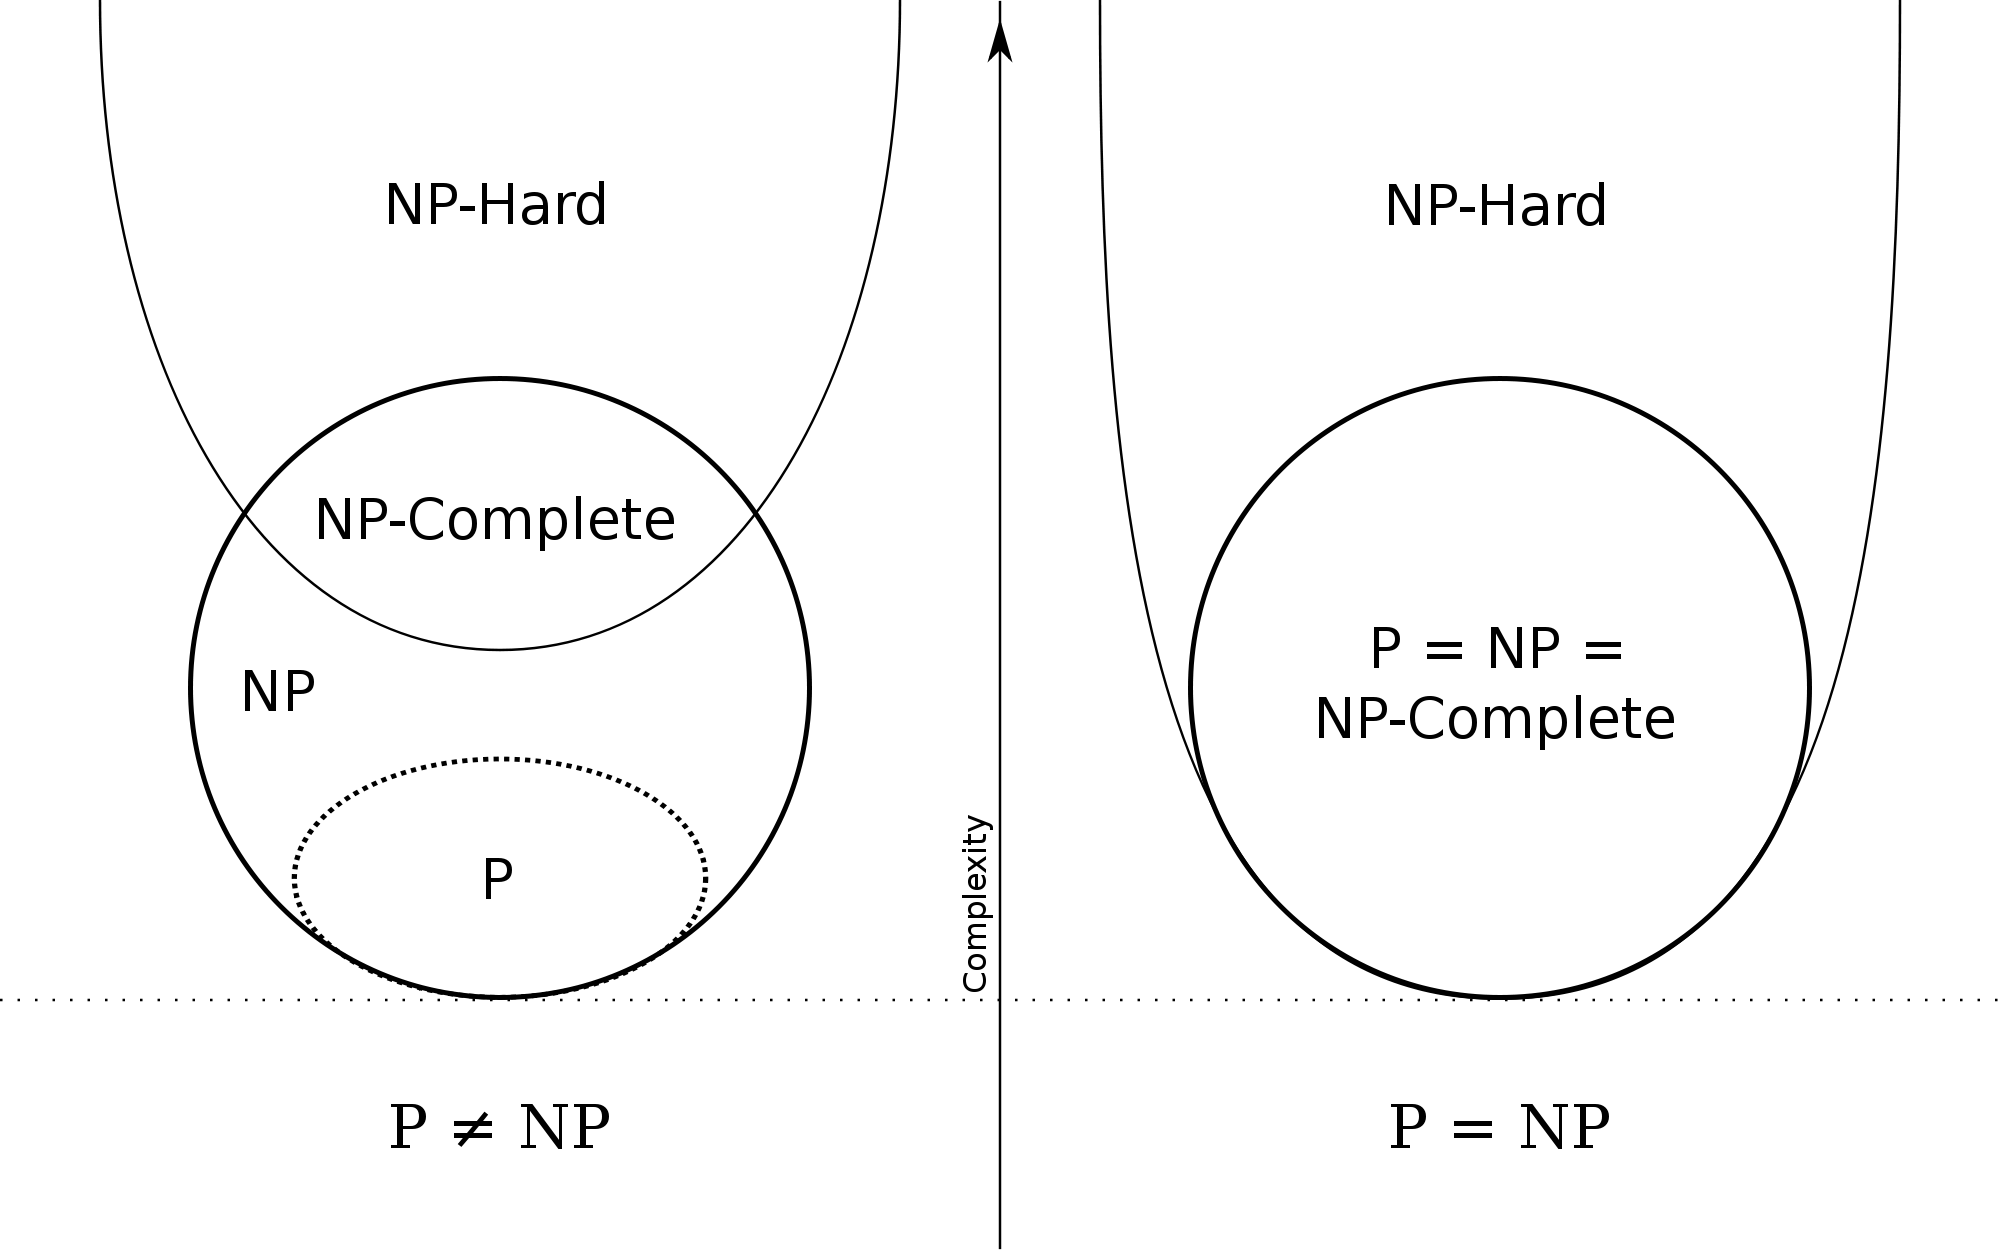
\includegraphics[width=0.8\linewidth]{complexity_venn}
  \caption{Sammenhenger mellom kompleksitetskategorier}
\end{figure}



%%%%%%%%%%%%%%%%%%%%%%%%%%%%%%%%%%%%%%%%%%%%%%%%%%%%%%%%%%%%
\section{NPC-problemer}
%%%%%%%%%%%%%%%%%%%%%%%%%%%%%%%%%%%%%%%%%%%%%%%%%%%%%%%%%%%%
\paragraph{Knapsack} Gitt en mengde gjenstander med tilordnet verdi og vekt, hvilken kombinasjon gir størst total verdi gitt en øvre vektgrense?
\subparagraph{1-0 Knapsack} Man kan kun ta med én eller ingen av hver gjenstand.
\paragraph{Subset-sum} Gitt en mengde tall, finn en delmengde som summeres til $0$. Spesialtilfelle av knapsack, kan mao. reduseres til knapsack: Subset-sum $\leqslant$ \mbox{knapsack}.
\paragraph{Vertex cover} Finn et mengde noder slik at alle kanter i en graf grenser til minst én node i mengden.
\paragraph{Hamiltonian path} En sti som besøker hver node presist én gang.
\paragraph{Travelling salesman} Minimal Ham-cycle i en komplett, vektet graf. NP-hard, ikke NP-komplett.
\paragraph{CIRCUIT-SAT} Finn en boolsk krets har et fast sett innganger som alltid gjør utgangen sann. Bevist å være NP-komplett.
\paragraph{SAT} Som CIRCUIT-SAT, men med et matematisk boolsk uttrykk. CIRCUIT-SAT kan reduseres til SAT og vice versa.
\paragraph{Max clique} En clique er en delgraf som er komplett. En max clique er den største cliquen i en graf. Merk at SAT $\leqslant$ CLIQUE. Eksempel: Finn grupper i et sosialt nettverk der alle kjenner hverandre.



%%%%%%%%%%%%%%%%%%%%%%%%%%%%%%%%%%%%%%%%%%%%%%%%%%%%%%%%%%%%
\section{Parallellprogrammering}
%%%%%%%%%%%%%%%%%%%%%%%%%%%%%%%%%%%%%%%%%%%%%%%%%%%%%%%%%%%%
\paragraph{Spawn} Nøkkelord som gjør et prosedyrekall som \textit{kan} kjøres parallelt.
\paragraph{Sync} Nøkkelord som pauser kjøring til alle barn kalt med \textbf{spawn} er ferdige.
\paragraph{$T_P$} Tiden en algoritme bruker når den kjøres på $P$ prosessorer.
\paragraph{Work} Work $= T_1$ er totalt arbeid, dvs. tiden algoritmen ville brukt på én prosessor.
\paragraph{Span} Span $= T_\infty$ er den lengste serielle utregningen, dvs. tiden algoritmen ville brukt gitt ubegrenset mange prosessorer.
\paragraph{Speedup} Speedup $= T_1 / T_P$ er hvor mye raskere beregningen går på $P$ kontra én prosessor.
\paragraph{Parallellitet} Parallellitet $= T_1 / T_\infty$ er et mål på i hvilken grad en beregning gjøres parallelt.



%%%%%%%%%%%%%%%%%%%%%%%%%%%%%%%%%%%%%%%%%%%%%%%%%%%%%%%%%%%%
\section{Masterteoremet}
%%%%%%%%%%%%%%%%%%%%%%%%%%%%%%%%%%%%%%%%%%%%%%%%%%%%%%%%%%%%
$$T(n) = aT\left(\frac{n}{b}\right) + n^c$$
\begin{enumerate}
\item $\log_b a < c \implies T(n) = \Theta(n^c)$
\item $\log_b a = c \implies T(n) = \Theta(n^c \log n)$
\item $\log_b a > c \implies T(n) = \Theta(n^{\log_b a})$
\end{enumerate}
\end{document}
